\documentclass[aspectratio=169,handout]{beamer}
\usepackage{borelian}

\begin{document}
    \classtitle{17}{Evaluación de modelos de aprendizaje no supervisado}{15 de enero de 2026}

    \begin{frame}{Motivación}
    A pesar de que los clústeres son más complejos de evaluar que los modelos de clasificación, es necesario saber su eficacia en la realización de su tarea.

    \pause
    \begin{itemize}
        \item ¿Qué pasa si las agrupaciones encontradas son aleatorias?
        \pause
        \item ¿Y si mis datos en realidad no tenían un patrón?
    \end{itemize}

    \pause
    La complejidad radica en que ahora no tenemos una interpretación directa, a diferencia del aprendizaje supervisado (la etiqueta asignada \textbf{está bien} o \textbf{no}).
    \end{frame}

    \begin{frame}{Tipos de métricas}
        La división de las métricas que se usan para evaluar la generación de clústeres se dividen principalmente en $3$ estrategias:

        \pause
        \begin{itemize}
            \item \underline{No supervisadas}: miden la calidad sin usar información externa (estadísticas como la inercia, cohesión, separación, etc.).
            \pause
            \item \underline{Supervisadas}: incorporan el conocimiento experto externo para determinar si los clústeres forman agrupaciones coherentes de los datos.
            \pause
            \item \underline{Relativas}: compara resultados entre distintas instancias de aplicación de un método. Por ejemplo, aplicar $K$-means dos veces, con diferentes inicializaciones de centroides, y comparar sus medidas de inercia.
        \end{itemize}
    \end{frame}

    \begin{frame}{Métricas no supervisadas}
        Se basan netamente en los datos; la estadística que se puede extraer desde ellos.

        \pause
        \begin{itemize}
            \item Suelen usar índices de cohesión, relacionados con la distancia intraclúster, y separación, relacionados con la distancia interclúster.
            \pause
            \item Pensando de manera general, la validez $V$ de un conjunto de $K$ clústeres se puede expresar como una validez ponderada por factores de peso $w$:
            \begin{equation*}
            V\left(\{C_1, \dots, C_K\}\right) = \sum_{i=1}^K w_i \cdot V(C_i)
            \end{equation*}
            \pause
            Si no nos interesa darle más relevancia a algún clúster, entonces la suma se simplifica a la suma de las valideces de cada uno.
        \end{itemize}
    \end{frame}

    \begin{frame}{Estrategias de mejora}
        \begin{itemize}
            \item Si un clúster tiene cohesión muy baja, podemos separarlo. Así mismo, si dos clústeres tienen una separación muy baja, podemos unirlos.
            \pause
            \item También podemos evaluar cuánto contribuye un punto en particular a la cohesión y separación de su clúster.
            \pause
            \item Una métrica que combina la cohesión con la separación es el coeficiente de Silhouette.
        \end{itemize}
        \pause
        \begin{figure}[H]
            \centering
            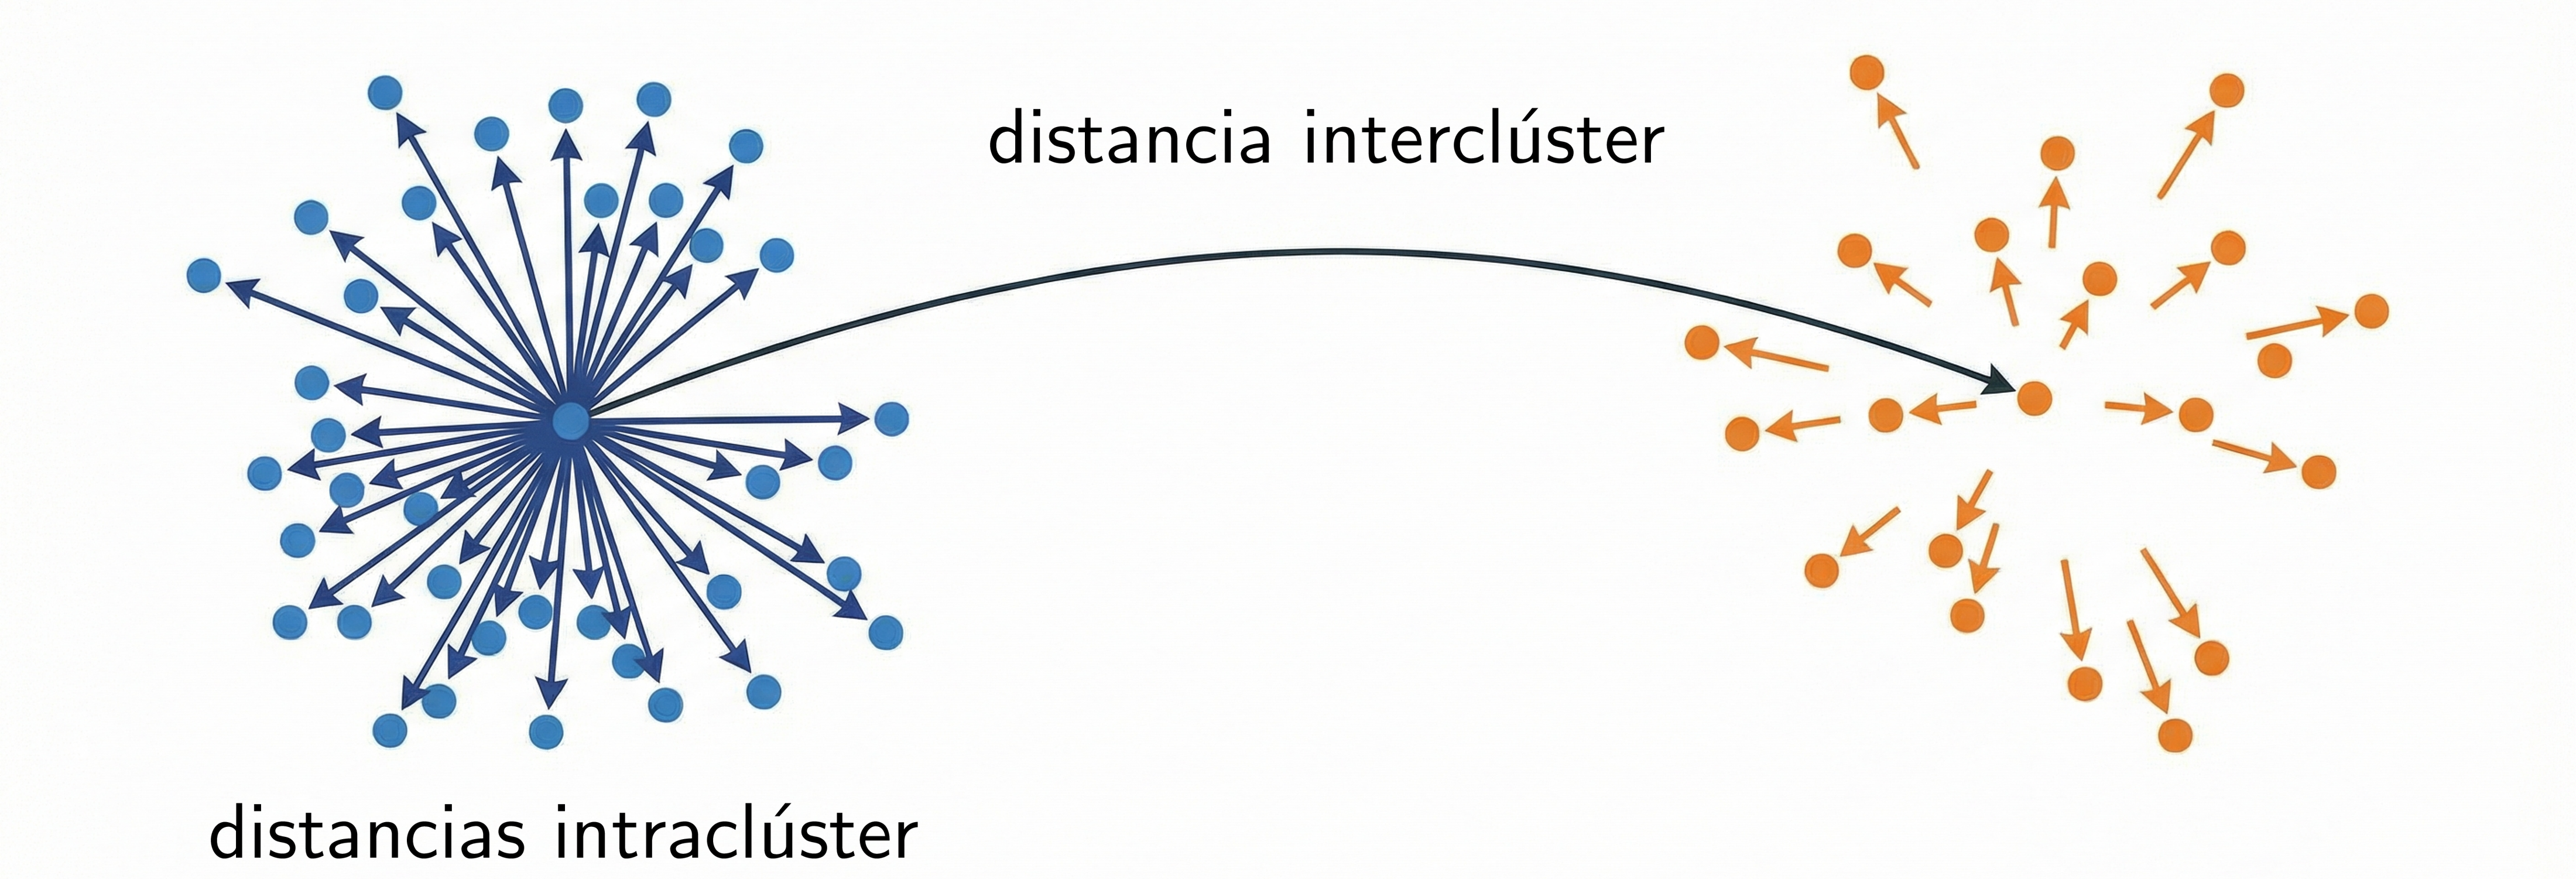
\includegraphics[width=.8\linewidth]{days/09/images/distances_intra_intercluster.png}
        \end{figure}
    \end{frame}

    \begin{frame}{Coeficiente de Silhouette}
        Para un punto individual, que denotaremos con la letra $i$:

        \pause
        \begin{enumerate}
            \item Se calcula $a_i$ como la distancia promedio de $i$ a los puntos de su clúster (llamémosle $C$):
            $$
            a_i = \frac{1}{|C|-1} \sum_{j \in C, j \neq i} d(i, j)
            $$

            \pause
            \item Se calcula $b_i$ como la mínima distancia promedio de $i$ a puntos de otro clúster (llamémosle $C'$):
            $$
            b_i = \min_{C' \in \mathcal{C}, C' \neq C} \frac{1}{|C'|} \sum_{j \in C'} d(i,j)
            $$

            \pause
            \item El coeficiente de Silhouette es $s_i = \frac{b_i - a_i}{\max\{a_i, b_i\}} \in [-1, 1]$. Mientras más cerca esté de $1$, mejor.
        \end{enumerate}
        
        \pause
        Esta idea se puede generalizar para calcular el coeficiente de Silhouette de un clúster, o incluso del conjunto total de clústeres.
    \end{frame}

    \begin{frame}{Métricas supervisadas}
        \begin{itemize}
            \item La información experta externa puede tener etiquetas, porque el grado de conocimiento adquirido por las personas en distintos campos lo permite.
            \pause
            \item Si tenemos ejemplos etiquetados, finalmente, podríamos ver la consistencia entre lo real y lo predicho por los clústeres.
            \pause
            \item De ser así, ¿cuál es el fin del aprendizaje no supervisado?
            \pause
            \begin{itemize}
                \item A veces, los patrones capturados por los clústeres pueden revelar comportamientos no triviales, por lo que es un buen complemento.
                \pause
                \item También, podemos saber si las técnicas de clusterización permiten generar grupos dado un problema que queremos resolver.
                \pause
                \item No siempre tenemos a mano varias etiquetas, podemos tener pocas, y usarlas sólo para validar...
            \end{itemize}
        \end{itemize}
    \end{frame}

    \begin{frame}{Métrica supervisada: entropía}
        Corresponde al grado en que un clúster en específico contiene ejemplos de una sola clase.

        \pause
        \begin{enumerate}
            \item Para cada clúster, calculamos la probabilidad de que un elemento $i$ del clúster pertenezca a la clase $j$: $p_{ij} = m_{ij}/m_i$, donde $m_i$ es el número de elementos en el clúster $i$, y $m_{ij}$ la cantidad de elementos de la clase $j$ en el clúster $i$.

            \pause
            \item Calculamos la entropía del clúster $i$, considerando que hay $C$ clases en total:
            $$
            e_i = -\sum_{j=1}^C p_{ij} \log_2 p_{ij}
            $$

            \pause
            \item Calculamos finalmente la entropía total del sistema, considerando que tenemos $K$ clústeres y $m$ datos en total. Esta métrica usa un ponderador de peso $m_i/m$, que corresponde a la proporción de elementos del clúster $i$ con respecto al total.
            $$
            e = \sum_{i=1}^K \frac{m_i}{m} \cdot e_i
            $$
        \end{enumerate}
    \end{frame}

    \begin{frame}{Métrica supervisada: pureza}
        Corresponde al nivel en que un clúster contiene elementos de una sola clase, usando la clase predominante.
        \pause
        \begin{itemize}
            \item Se calcula como la probabilidad máxima de una de las $C$ clases. Para un clúster $i$:
            $$
            \text{pureza}(C_i) = \max_{j \in \{1, \dots, C\}} p_{ij}
            $$
            \pause
            \item Al igual que la entropía, la pureza total del sistema es un promedio ponderado, donde el ponderador corresponde a la proporción de elementos de cada clúster con respecto al total.
            $$
            \text{pureza}(\{C_1, \dots, C_K\}) = \sum_{i=1}^K \frac{m_i}{m} \cdot \text{pureza}(C_i)
            $$
        \end{itemize}
    \end{frame}

    \begin{frame}{Significancia de las medidas supervisadas}
        No es fácil interpretar estos puntajes, pero nos otorgan una guía para entender la calidad de los clústeres generados.
        \pause
        \begin{itemize}
            \item Una pureza de $0$ indica una agrupación deficiente, mientras que una pureza de $1$ sugiere una buena agrupación.
            \pause
            \item Lo contrario sucede para la entropía y la inercia, donde valores bajos indican una mejor agrupación.
        \end{itemize}
    \end{frame}

    \begin{frame}{Validación con expertos e iteración}
        \begin{itemize}
            \item La validación con expertos implica evaluar los clústeres para determinar si producen un resultado esperado.
            \pause
            \item Ellos nos pueden decir, dadas las descripciones que nosotros tengamos de los clústeres, si las relaciones que se establecen en los grupos tienen sentido y por qué.
            \pause
            \item Es importante iterar si se encuentran inconsistencias. Existen muchos motivos por los cuales el resultado pudo haber sido deficiente (p. ej., \emph{garbage-in}, \emph{garbage-out}, o escoger un método inadecuado).
        \end{itemize}
    \end{frame}
\end{document}